\section{Experimental methods and apparatus}\label{sec:experimental-technique-and-apparatus}
To examine the diffraction pattern from different slit patterns (and eventually a helix) we use the system described in Figure~\ref{fig:Apparatus}.
\begin{figure}[H]
    \centering
    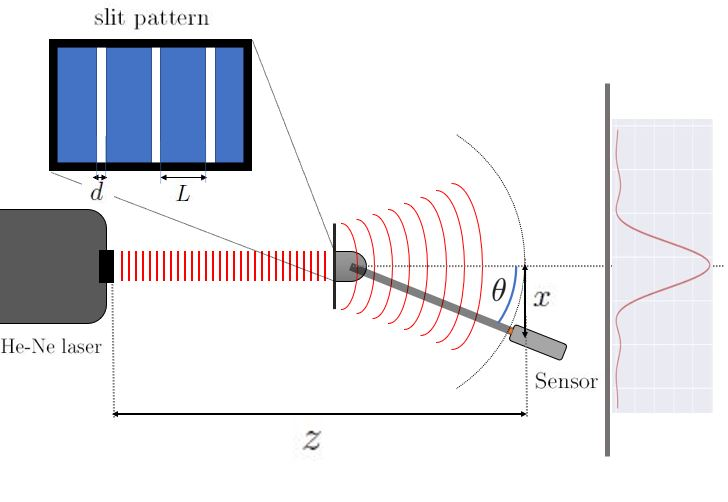
\includegraphics[width=0.9\columnwidth]{figures/Apparatus.JPG}
    \caption{A description of the system used to measure the intensity of light coming from a He-Ne laser at different angles. An example of a slit
    pattern is shown, but can be swapped for any diffracting object}
    \label{fig:Apparatus}
\end{figure}
Where the He-Ne laser produces an approximately monochromatic plane wave with $\lambda=632.8 [nm]$ and
We also note that the sensor has an iris through which the light goes before measured, thus all light within that width is accounted for when measuring a
certain angle.
Taking into account the "Iris effect" our expected intensity is then $I(x)=\int\limits_{x-d}^{x+d}I(x')dx'$.
For the helix we use a similar set up, removing the sensors, replacing the slit pattern with the helix and changing the distance from the screen to $z=1.9[m]$.
The measurement was then taken with a camera, and to analyse this diffraction pattern we take different sections of the photo and treat them as diffraction caused by different sections of the helix.
Much like the iris effect in our photoelectric sensor the camera we used not only has a 2-dimensional iris which causes a similar effect, but there's also the effect of "focus".
The camera's focus determines the distance for which a pixel describes the light that comes from the smallest area, simply put - distance of sharpest image.
Since our camera was placed at some angle relative to the laser beam, we measured diffraction at different distances from the camera and therefore could only focus on a single point of the diffraction pattern.

